\section{Sensor Interface Board}
\label{sec-sensorinterfaceboard}
\label{subsec-signalhardware}

\begin{figure}[t] 
\begin{center} 
\includegraphics[width=0.9\hsize]{./figs/EWSN2005/2005-VolcanoMote.eps}
\end{center} 
\caption{{\bf 2004 Volcano Mote.}
A Mica2 mote with simple sensor interface board allowing a single microphone
to be attached as shown.}
\label{fig-2004volcanomote}
\end{figure}

Of any system component, the hardware interface board received the most
significant internal redesign on the way to our second deployment in 2005.
Our proof-of-concept deployment deployed nodes fitted with a simple hardware
interface board interfacing the Mica2 motes at use at the time with a single
microphone.  The Mica2's 10~bit ADCs were used to collect acoustic signals at
100~Hz, the sampling rate necessary to capture volcanic infrasound.  Sampling
was driven by the Mica2's onboard oscillator and the standard TinyOS
\texttt{Timer} component. Figure~\ref{fig-2004volcanomote} shows a Mica2 mote
with the hardware interface board attached.

In particular, the following set of limitations of the original board had to
be addressed in order to provide the datum quality required by the
scientists:

\begin{enumerate}
\item {\bf Resolution:} Scientific analysis required a per-sample resolution
of at least 16~bits, with greater than 20 being ideal. The Mica2 motes used
for the original deployment provided only 10~bits of resolution and later
designs, such as the TelosB, provided only 16.
\item {\bf Filtering:} The ideal filter for the seismic and infrasonic data
our nodes were collecting is a hard cutoff at 50~Hz. Unfortunately, upon
review the original sampling board had a passive filter with a 3~dB point of
5~Hz which meant that desirable components of the signal were being
attenuated.
\item {\bf Number of Channels:} Fitting each node with both seismometers and
microphones, as we wanted to do for the second deployment, required allowing
multiple sensors to be attached to each node. Our original board was built to
interface a single sensor.
\item {\bf Timing:} We expected that providing the high-fidelity timing
necessary to track fast-moving pressure waves across the network would
require both a stable timing source driving the per-node sampling and a way
of interpreting local times across multiple nodes.  Multi-hop time
synchronization is discussed separately below, but the timing process
necessitated a stable local source that would produce clean per-sample
intervals.
\item {\bf Isolation:} When testing our Tungurahua deployment before fielding
it we noticed that, due to poor isolation between multiple chips on the
Mica2, radio transmissions were interfering with signal collection. The large
amount of current required to drive the CC1000 radio was flooding the ground
plane and causing the onboard ADC voltage reference to shift. While our
original system worked around this crudely in software, providing clean data
for scientists would require isolating the sampling components from sources
of potential interference.
\end{enumerate}

\subsection{2005 Board Redesign}
\label{sec-2005-board}

\begin{figure}[t]
\begin{center}
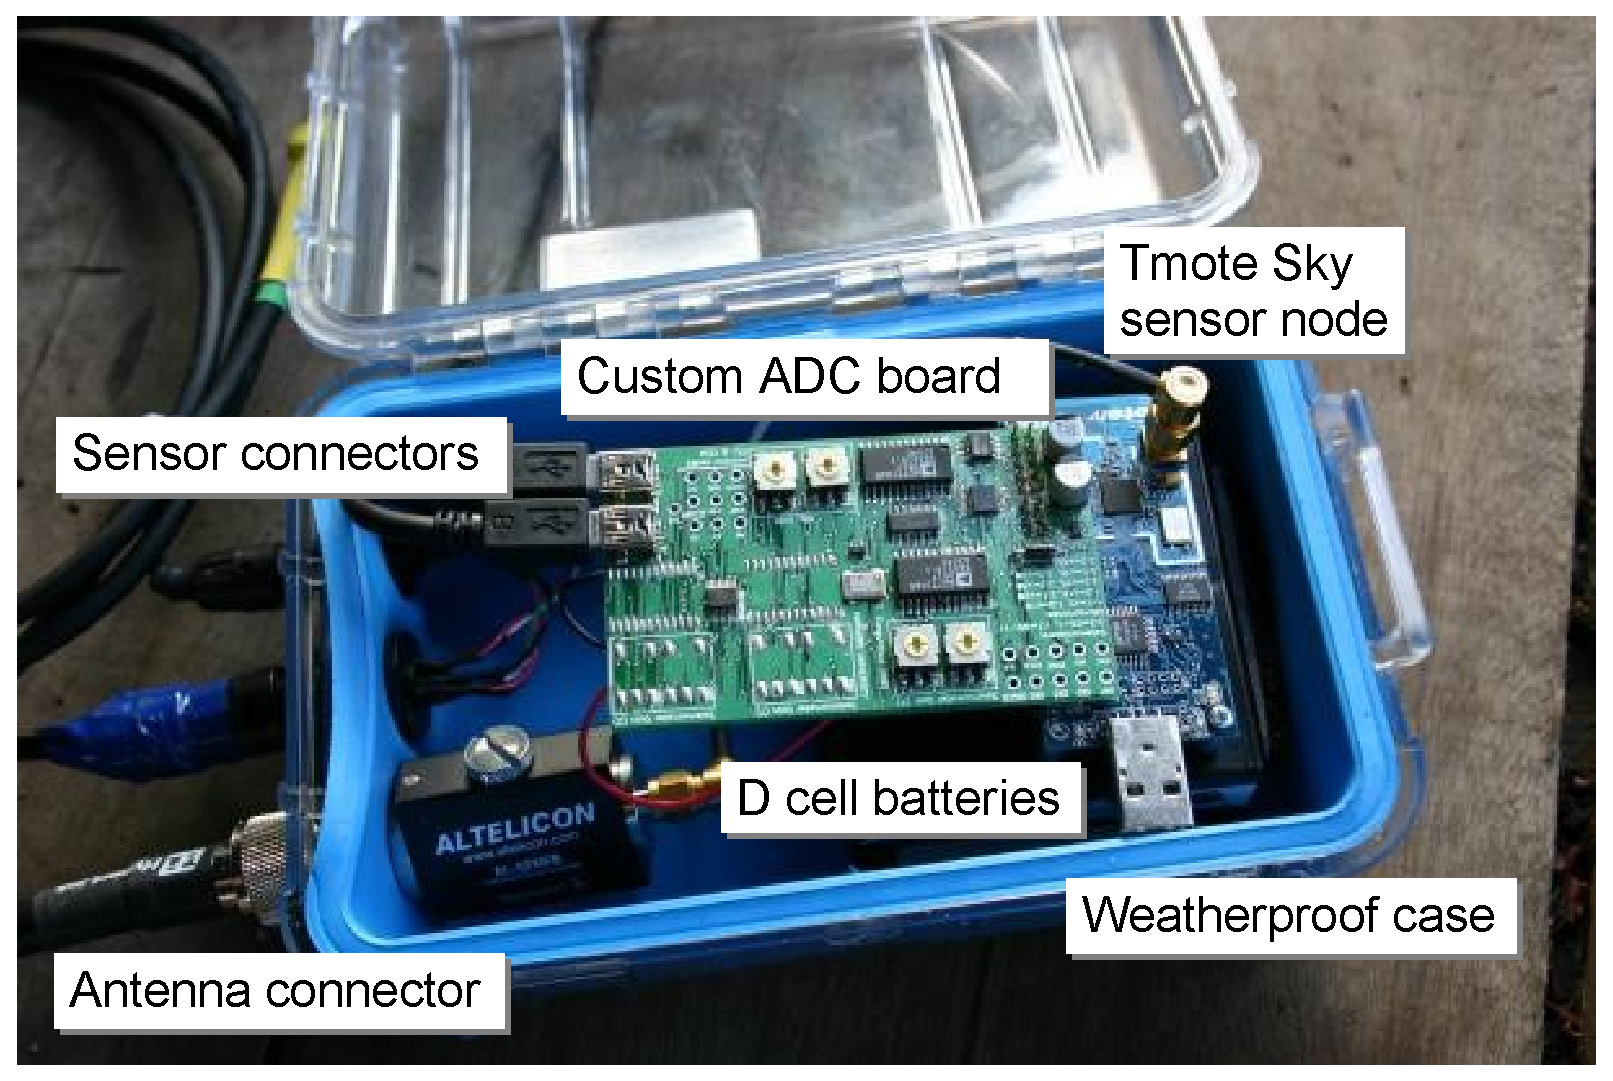
\includegraphics[width=1.0\hsize]{./figs/OSDI2006/2006-VolcanoMote.eps}
\end{center}
\caption{{\bf The second iteration of our volcano monitoring sensor
node, fielded at Reventador in 2005 and Tungurahua in 2007.}}
\label{fig-2005volcanomote}
\end{figure}

Initially, we considered using the TMote Sky's onboard ADCs.  The TMote had a
single 16~bit ADC --- which we believed to be well-isolated from other
circuitry on the node --- and the ability perform DMA sampling from the ADC
into onboard RAM while leaving the CPU in a low-power state.  However,
several limitations of the TMote led us towards a standalone board. First,
the 16~bit resolution of the onboard ADC was not quite enough to support our
application. Had this been the sole limitation we may have settled for
16~bits, but a separate board meant we could select higher-resolution ADCs.
In addition, the TMote had a \textit{single} 16~bit ADC, and we were worried
about multiplexing this between multiple channels.  Second, we were concerned
with providing a stable filter centered at 50~Hz.  Building a passive filter
at that low of a frequency is difficult, so we concluded that the filtering
would have to be done by an oversampling ADC.  Performing the filtering on
the TMote would have required oversampling at rates it was not capable of.

For these reasons we moved to a standalone sensor interface board providing
its own reference voltage (ensuring isolation), ADCs (allowing us to choose
the resolution and number of channels and implement digital filtering), and
clock source (ensuring a highly-accurate sampling rate).  Offloading this
much functionality to a hardware board was risky since it left us little room
for error in the design and fabrication, but it significantly simplified the
code running on the nodes themselves.  As it turned out, the fully
built-out application we deployed at Reventador Volcano consumed almost all
of the TMote Sky's 48~kB of program memory, leaving little room for the
functions we offloaded to the interface board.

As deployed in 2005 we were quite happy with the performance of our external
sensor interface board. The analysis conducted and reported
here~\cite{volcano-osdi06} showed no significant deficiencies in the board
design.  There was some initial confusion about the sampling rate which, due
to the precision of the oscillator and the settings on the ADC, turned out to
be slightly less than exactly 100.000~Hz, but it was extremely consistent
across multiple nodes meaning that data collected from several stations could
be lined up and processed together.  We designed software allowing us to
modify the ADC settings on-the-fly and this came in handy during the
deployment when we realized that the hardware gain settings were too low. We
were able to modify them in software and address the problem without
returning to the deployment site.

%\subsection{Interfacing to the TMote Sky}
%
%Once we chose to fabricate our own board several other questions emerged.
%First, how would we interface our board to the TMote itself?  Second, how
%configurable did we want the sensor interface board to be?
%
%The first question we resolved in favor of choosing ADCs featuring a simple
%serial interface that could be manually-clocked (i.e. ``bit banged'') to
%clock out samples.  While a high-speed bus such as SPI or I2C would have
%greatly sped up the communication between node and board, we were concerned
%about arbitrating the multiple devices sharing these buses already and chose
%to further separate our hardware board onto its own dedicated communication
%lines. This decision, however, led to a tradeoff in terms of the
%configurability of the device, since we were limited by the number of
%available pins on the headers exposed by the TMote Sky.  By using all
%available externally-exposed pins we were able to operate and configure the
%external ADCs, but the small number of pins led to the exclusion of some
%seemingly obvious functionality. For example, there was no way to turn the
%entire sampling board on or off, which a more intelligent node might have
%wanted to do to save power, or to reset the sampling board components to a
%known good state. Additionally, due to an overlap between two pins
%configuration settings on the ADCs --- such as the sampling rate and internal
%gain --- could be written, but not read.
%
%As far as configurability the ADC that we chose exposed a number of different
%settings that we found useful. In particular, in the field we used the
%internal gain setting on the ADCs to work around a poor choice of hardware
%gain settings on the hardware board itself. Hardware gain settings, which
%could be controlled through rotational switches, were another element of
%configurability we included on the board itself.  Unfortunately, as it
%happened local testing using the seismometers and microphones we deployed led
%us to choose an overly insensitive set of gain settings to canonicize on the
%board itself. When the system was fielded and collected data showed the
%hardware gain settings, even at their highest, to be too low, we were able to
%change the ADC's internal gain using a software command.  Because changing
%the internal gain damaged the effective resolution of the ADC, we were happy
%at that point to have deployed an ADC wider than what was strictly necessary.
%The ADCs also included a number of different configuration parameters that,
%while potentially useful, we never explored, such as the ability to change
%the sampling rate.


\subsection{Performance and Future Designs}

The external interface board was not without its drawbacks. In particular,
the oversampling ADCs we chose consumed a large amount of power, around 8~mA
per ADC.  When combined with other board components, such as the reference
voltage, 3 to 5V conversion necessary to power certain components, and
external oscillator, the sensor interface board ended up consuming around
60~mA of current, or around 3 times more than the TMote with radio and CPU
fully active.  As mentioned previously, there is no way to power down the
interface board remotely, nor would we be able to without immediately losing
data since the ADCs are sampling at tens of kHz.  For the Reventador
deployment we provisioned around this high power consumption by deploying
larger (D~cell) batteries and replacing them several times.  This can be seen
as a tradeoff between datum quality --- which necessitates the high-power
external sensor interface board --- and a reduction in dataset quality
through shorter systems lifetimes or higher-duty cycles due to increased
power consumption.

It is likely that the next iteration of this board will take on several
additional challenges. First, we will strive to lower the power consumption
while maintaining high fidelity through the use of newer ADCs which can hold
down their current consumption even while performing the several factors of
oversampling necessary to perform digital filtering.  Second, we are
increasingly interested in the ability to support multiple applications.
Thus any future sensor board design, either built in-house or purchased
as-is, will be expected to support multiple applications and sensor types.
Our current board is, in its choice of ADCs and hardware-filtering,
somewhat tailored to the volcano application. We'd like to move away from
this if possible.

These two future goals are in many ways at odds with each other, since the
challenge of reducing the power consumption of a board designed for a very
specific purpose is different and potentially more manageable than the
challenge of designing a general-purpose yet low power board. This is a
design tension that we expect to continue to play out in future hardware
revisions.
